\chapter{Desenvolvimento}
\label{desenvolvimento}
Neste capítulo, será descrita o desenvolvimento e as soluções da implementação do WiSync para este trabalho.

A versão do WiSync entregue com este texto foi escrita em Python \cite{python}, versão 2.7, linguagem de programação interpretada originalmente lançada em 1991.
Python foi escolhida por sua facilidade na implementação e extensa disponibilidade de bibliotecas de código aberto.

Originalmente, havia como objetivo tornar o programa compatível com os três sistemas operacionais mais comuns do mundo: Microsoft Windows, Apple OS X e Linux.
Contudo, devido a diferenças inerentes na forma como o Windows funciona, optou-se por manter apenas compatibilidade com OS X e Linux.
Para tal, o WiSync foi desenvolvido usando os seguintes computadores para testes:

\begin{center}
  \begin{tabular}{ l | l | l }
    \hline
    \textbf{Nome} & ``SgtPepper'' & ``Packard'' \\ \hline \hline
    Sistema Operacional & OS X 10.11 & Linux Mint 17 \\ \hline
    Processador & Intel Core i5-4308U & Intel Core i7-2600 \\ \hline
    RAM & 8GB DDR3L & 8GB DDR3 \\ \hline
    Armazenamento & SSD 512GB & HDD 320GB \\ \hline
    Conectividade & Wi-Fi 802.11n 5GHz & Cabo Ethernet \\ \hline
    IP local & 192.168.1.110 & 192.168.1.132 \\
    \hline
  \end{tabular}
\end{center}

\section{Bibliotecas Usadas}
Para executar o WiSync, são necessárias algumas bibliotecas padrão do Python: \texttt{os}, \texttt{sys}, \texttt{argparse}, \texttt{time}, \texttt{json}, \texttt{datetime}.
Também é usada uma versão modificada do programa \texttt{woof.py} \cite{woof} (distribuída sob a licença GNU General Public License), que é usada na hora de transmitir os arquivos entre os computadores.
No WiSync, arquivos JSON são usados para armazenar e transmitir as listas de arquivos geradas pela leitura e comparação dos diretórios.

\subsection{Mudanças feitas ao woof}
Como citado anteriormente, o programa \texttt{woof.py} \cite{woof} foi usado como biblioteca para auxiliar no envio de arquivos por HTTP.
Para se adequar às necessidades do WiSync, algumas pequenas mas importantes mudanças tiveram que ser feitas:
\begin{itemize}
  \item Após servir um arquivo ao outro computador, o endereço IP do computador remoto é armazenado para poder ser utilizado novamente no futuro sem depender de outras buscas por endereços.
  \item Originalmente, o \texttt{woof.py} utilizava diversas \textit{threads} para permitir o \textit{download} simultâneo de arquivos. Como essa funcionalidade não é necessária para o WiSync e as múltiplas \textit{threads} causavam consequências indesejadas, o código foi alterado para desabilitar isso. 
\end{itemize}

\section{Situações consideradas}
Tratando-se das possíveis diferenças que podem existir entre um par de diretórios (vamos chamá-los de A e B), as seguintes possibilidades são consideradas:
\begin{itemize}
  \item Arquivos existem em A mas não em B e vice-versa. Como demonstrado na figura \ref{a}, nessa situação basta copiar os arquivos do diretório que os contém para o que não os contém.
  \begin{figure}[h]
    \centering
    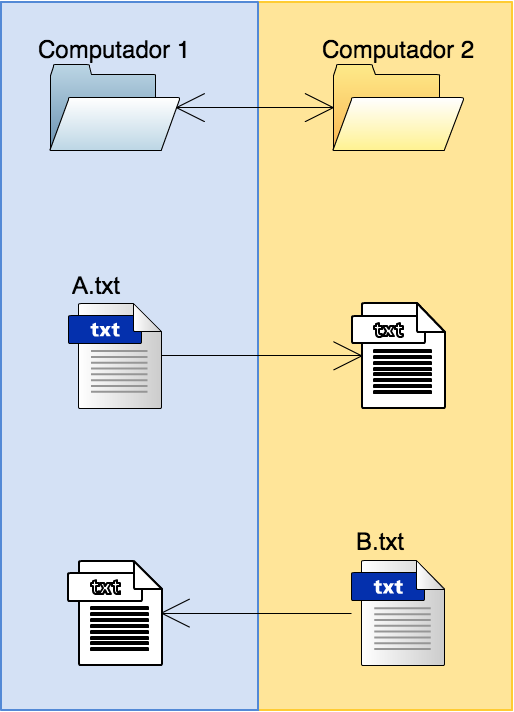
\includegraphics[width=200pt]{img/a.png}
    \caption{Caso onde os dois diretórios têm arquivos novos}
    \label{a}
  \end{figure}
  \item Arquivos com o mesmo nome existem em A e B mas têm conteúdo diferentes. Caso da figura \ref{b}. Nesse caso o WiSync utiliza o histórico da última sincronização antes da atual e as informações de data de modificação dos arquivos. Se o arquivo já existia antes e a data de alteração de uma das versões atuais é igual à anterior (implicando que o arquivo não foi modificado desde então), a versão mais recente substitui a mais antiga. O mesmo processo se aplica a um arquivo que foi excluído desde a última sincronização.
  \begin{figure}[h]
    \centering
    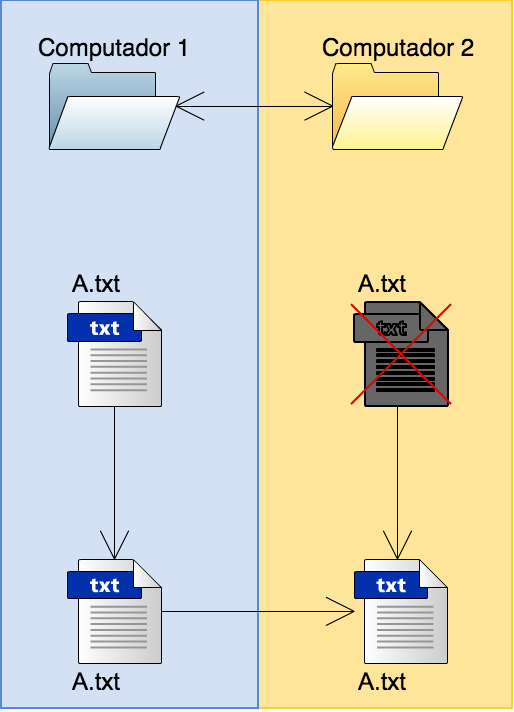
\includegraphics[width=200pt]{img/b.png}
    \caption{Caso onde um arquivo foi atualizado em apenas um dos diretórios}
    \label{b}
  \end{figure}
  \item Similar à situação acima, mas ambos arquivos têm datas de modificação diferentes às da última sincronização, ou não há informação sobre a última sincronização. Nesse caso, mostrado na figura \ref{c}, o WiSync copia ambas versões para o outro diretório, renomeando os arquivos para evitar conflitos e sobre-escritas.
  \begin{figure}[h]
    \centering
    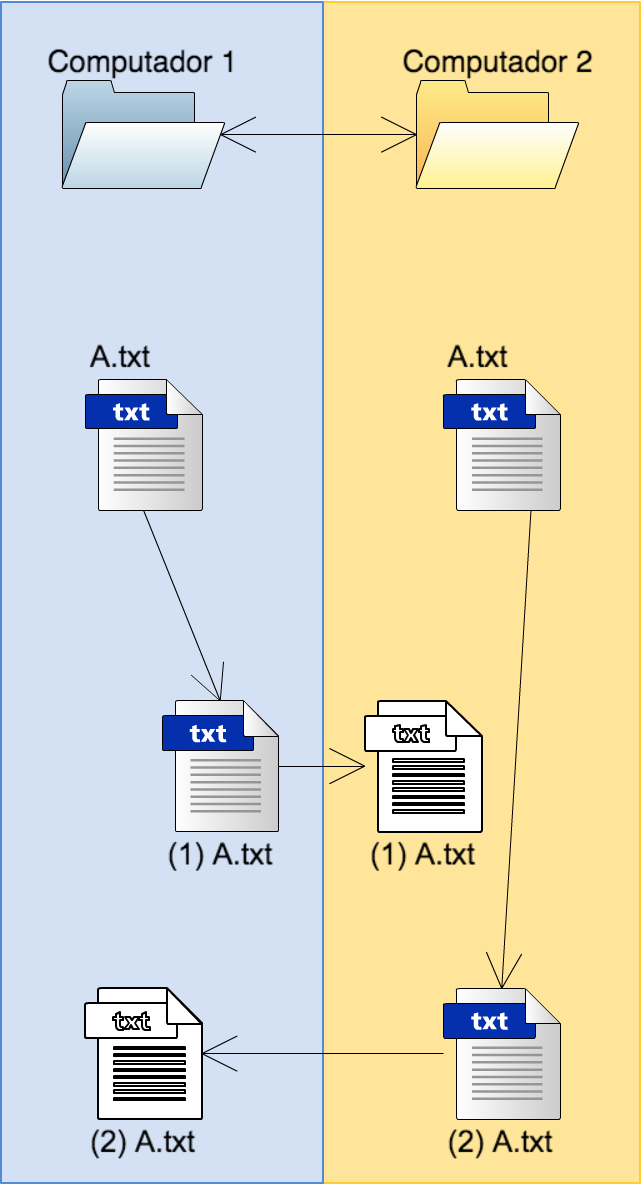
\includegraphics[width=200pt]{img/c.png}
    \caption{Caso onde há conflito de versões entre dois arquivos}
    \label{c}
  \end{figure}
  \item Caso um arquivo seja renomeado, o WiSync tratará essa situação como se fossem dois arquivos: um excluído e um novo. Caso o arquivo correspondente no diretório remoto não tenha sido alterado desde a última sincronização, este será excluído e uma nova cópia, com o novo nome, será criada. Isso é ilustrado na figura \ref{d}
  \begin{figure}[h]
    \centering
    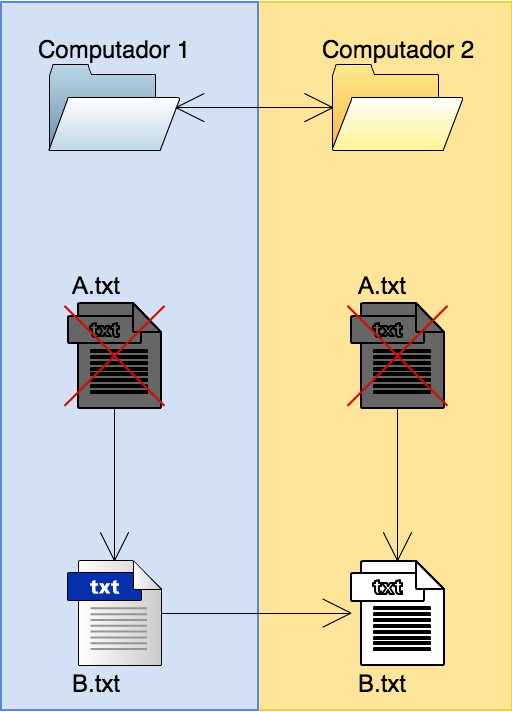
\includegraphics[width=200pt]{img/d.png}
    \caption{Caso onde um arquivo foi renomeado}
    \label{d}
  \end{figure}
\end{itemize}

\section{Fluxo do programa}
Durante a execução, o WiSync executa as seguintes operações:
\begin{enumerate}
  \item Processa parâmetros e configura as classes WiFiles e WiNet, que preparam o que é necessário para lidar com arquivos e rede no programa.
    \item As duas instâncias do programa trocam os arquivos JSON contendo informações sobre o diretório a ser sincronizado.
    \item Uma das instâncias utiliza esses arquivos JSON e, se existir, o arquivo contendo informações do estado anterior do diretório para gerar um novo JSON contendo a lista de arquivos que devem ser transferidos ou excluídos em cada um dos diretórios.
    \item A instância que realizou a comparação começa a enviar os arquivos de acordo com a lista contida no JSON e, ao mesmo tempo, a outra instância recebe esses arquivos.
    \item As instâncias trocam e a segunda passa a enviar arquivos para a primeira.
    \item Ambas instâncias excluem seus próprios arquivos de acordo com o JSON.
    \item Um novo JSON é gerado contendo as informações dos diretórios após a sincronização, que será usado para sincronizações futuras.
\end{enumerate}

\section{Dificuldades encontradas}
Durante o desenvolvimento do WiSync, algumas dificuldades foram encontradas.
A seguir elas são descritas e são apresentadas as soluções encontradas.

\subsection{Waits e timeouts}
Talvez a parte mais difícil do desenvolvimento do WiSync tenha sido levar em consideração o fato de que o programa roda em dois computadores diferentes, com velocidades diferentes e que se comunicam apenas ocasionalmente através da troca de arquivos.
Para evitar erros, é necessário garantir que ambos computadores estejam no mesmo passo ao mesmo tempo.

Um erro que aconteceu com frequência durante o desenvolvimento, por exemplo, é que um computador procurava o arquivo do outro antes deste ter preparado a hospedagem do arquivo.
Ou seja, o arquivo não estava disponível ainda e o primeiro computador retornava um erro de endereço inválido.
Para evitar isso, foi adicionado uma pausa de 1 segundo logo antes de tentar acessar um arquivo do outro computador.
Este tempo permite que o outro computador termine de preparar a hospedagem.
Essa solução não é infalível, pois pode ser que o computador demore mais ainda para hospedar e, neste caso, o erro acontece de qualquer forma.
Uma solução para isso seria criar um laço onde se tenta diversas vezes acessar o arquivo remoto mas, nos testes, isso teve um desempenho pior do que a pausa.

\subsection{Datas de criação/modificação}
Como explicado anteriormente, o WiSync utiliza metadados dos arquivos \-- a data modificação em particular \-- para decidir quais devem ser copiados.
Contudo, isso gerou um problema que não havia sido previsto: quando um arquivo é copiado para o outro, a data de modificação da cópia é a data de sincronização \-- não a data de modificação do arquivo original.
Ou seja, numa sincronização subsequente, a cópia é entendida como uma versão nova do arquivo e copiada novamente para o computador original.

Para resolver isso, foi usada a função \texttt{os.utime} do Python, dessa forma configurando as datas de criação e modificação do arquivo criado para serem iguais às do arquivo de origem. Uma preocupação que surgiu em relação a isso foi a possibilidade de, devido a configurações diferentes entre os computadores, um arquivo ter data de criação e/ou modificação futura ao relógio do sistema.
Contudo, testes foram realizados no Linux e no OS X e isso não se mostrou um problema.

\subsection{Ordem dos arquivos}
As listas de arquivos que o WiSync são armazenadas usando o tipo Dictionary, do Python, para que torne-se simples indexar os arquivos utilizando os nomes deles.
Contudo, um dicionário, ao ser percorrido, não tem uma sequência definida a ser seguida. 
ortanto, na hora de enviar e receber arquivos, o dicionário é convertido para uma lista de tuplas, ordenada alfabeticamente com os nomes dos arquivos.
Isso garante que ambos computadores enviem e recebam arquivos na mesma ordem.